\section{The Scattering Transform} \label{sec:ch4:scatternet}
While we have introduced the scattering trasnform before, we clarify the format
we use for this chapter's analysis. 

We use the $\DTCWT$ based scatternet introduced in the previous chapter 
\autoref{alg:ch3:dtcwt_scat} as a front end, with $K=6$ orientations, $J=2$
scales and $M=2$ orders. Consider a single channel input signal $x(\xy)$, $\xy
\in \reals[2]$.

The zeroth order scatter coefficient is the lowpass output of a $J$
level FB: 
\begin{equation}
  S_0x(\xy) \definedas x(\xy) \conv \phi_J(\xy)
\end{equation}
This is approximately invariant to translations of up to $2^J$ pixels\footnote{From here on,
we drop the $\xy$ notation when indexing $x$, for clarity.}. In exchange for
gaining invariance, the $S_0$ coefficients have lost information
(contained in the rest of the frequency space). The remaining energy of $x$ is
contained within the first order \emph{wavelet} coefficients:
\begin{equation}
  W_1x(\xy, j_1, \theta_1) \definedas x \conv \psi_{j_1, \theta_1}
\end{equation}
for $j_1\in\{1, 2\}, \theta_1\in\{15\degs, 45\degs \ldots, 165\degs\}$ (we may 
sometimes index $\theta$ with $1 \leq k \leq K$). We will want to
retain this information in these coefficients to build a useful classifier.

Let us call the set of available scales and orientations $\Lambda_1$ and use
$\lambda_1$ to index it. For both Morlet and $\DTCWT$ implementations, $\psi$
is complex-valued, i.e., $\psi = \psi^r + j\psi^i$ with $\psi_r$ and $\psi_i$
forming a Hilbert Pair, resulting in an analytic $\psi$.
 This analyticity provides a source of invariance --- small input shifts in $x$
 result in a phase rotation (but little magnitude change) of the complex wavelet
 coefficients\footnote{In comparison to a system with purely real filters such
 as a CNN, which would have rapidly varying coefficients for small input shifts
 \cite{kingsbury_complex_2001}.}.

Taking the magnitude of $W_1$ gives us the first order \emph{propagated}
signals:
\begin{equation}
  U_1x(\lambda_1, \xy) \definedas |x \conv \psi_{\lambda_1}| 
    = \sqrt{(x \conv \psi^r_{\lambda_1})^2 + (x \conv \psi^i_{\lambda_1})^2}
\end{equation}
The first order scattering coefficient make $U_1$ invariant up to 
the coarsest scale $J$ by averaging it:
\begin{equation}
  S_1x(\lambda_1, \xy) \definedas |x \conv \psi_{\lambda_1}| \conv \phi_J
\end{equation}
This has $KJ = 6\x 2 = 12$ output channels for each input channel. Later in this
chapter we will want to distinguish between the first and second scale
coefficients of the $S_1$ terms, which we will do by moving the $j$ index
to a superscript. I.e., $S_1^1$ and $S_1^2$ refer to the set of 6 $S_1$ terms
at the first and second scales.

Higher order scattering coefficients recover the information lost by
averaging $U_1$, and are defined as:
\begin{eqnarray}
  W_{m} &=& U_{m-1} \conv \psi_{\lambda_{m}} \\
  U_{m} &=& |W_{m}| \\
  S_{m} &=& U_m \conv \phi_J
\end{eqnarray}

Previous work shows that for natural images we get diminishing returns after
$m=2$. The second order scattering coefficients are defined only on paths of
decreasing frequency\cite{bruna_invariant_2013} as:
\begin{equation}
  S_2x(\lambda_1, \lambda_2, \xy) \definedas ||x \conv \psi_{\lambda_1}|
  \conv \psi_{\lambda_2}| \conv \phi_J
\end{equation}
As we only go on the paths of decreasing frequency $j_1 = 1$, $j_2=2$. This then
has $6\x6 = 36$ output channels per input channel.

Our output is then a stack of these 3 outputs:
\begin{equation}
  Sx = \{S_0x, S_1x, S_2x\}
\end{equation}
with $1+12+36=49$ channels per input channel.

\subsection{Scattering Colour Images}\label{sec:ch4:colour}
A wavelet transform like the $\DTCWT$ accepts single channel input, while we
often work on RGB images. This leaves us with a choice. We can either:
\begin{enumerate}
  \item Apply the wavelet transform (and the subsequent scattering operations)
    on each channel independently. This would triple the output size to $3C$.
  \item Define a frequency threshold below which we keep colour information, and
    above which, we combine the three channels.
\end{enumerate}
The second option uses the well known fact that the human eye is far less sensitive 
to higher spatial frequencies in colour channels than in luminance channels. 
This also fits in with the first layer filters seen in the well known
Convolutional Neural Network, AlexNet. Roughly one half of the filters were low
frequency colour `blobs', while the other half were higher frequency, greyscale,
oriented wavelets. 

For this reason, we choose the second option for the
architecture described in this chapter. We keep the 3 colour
channels in our $S_0$ coefficients, but work only on greyscale for high orders 
(the $S_0$ coefficients are the lowpass bands of a J-scale wavelet transform, so
we have effectively chosen a colour cut-off frequency of $2^{-J} \frac{f_s}{2}$).

We combine the three channels by modifying our magnitude operation from \eqref{eq:ch3:magbias} 
to now be:
\begin{equation}\label{eq:ch4:colour_mag}
 r_s = \sqrt{x_r^2 + y_r^2 + x_g^2 + y_g^2 + x_b^2 + y_b^2 + b^2} - b
\end{equation}
Where $x_r, x_g, x_b$ are the real parts of the wavelet response for the red,
green and blue channels, and $y$ is the corresponding imaginary part. This only
affects the $S_1$ coefficients, and the $S_2$ coefficients then are calculated
as normal. 

An alternative to \eqref{eq:ch4:colour_mag} is to simply combine the colours
before scattering into a luminance channel. However we choose to use \eqref{eq:ch4:colour_mag}
instead as this has the ability to detect colour edges with constant luminance.

With $J=2$ the resulting scattering output now has $3 + 12 + 36 = 51$ channels at $1/16$ the
spatial input size.

\section{The Inverse Scatter Network}\label{sec:ch4:descatternet}
\begin{figure}[t]
  \centering
  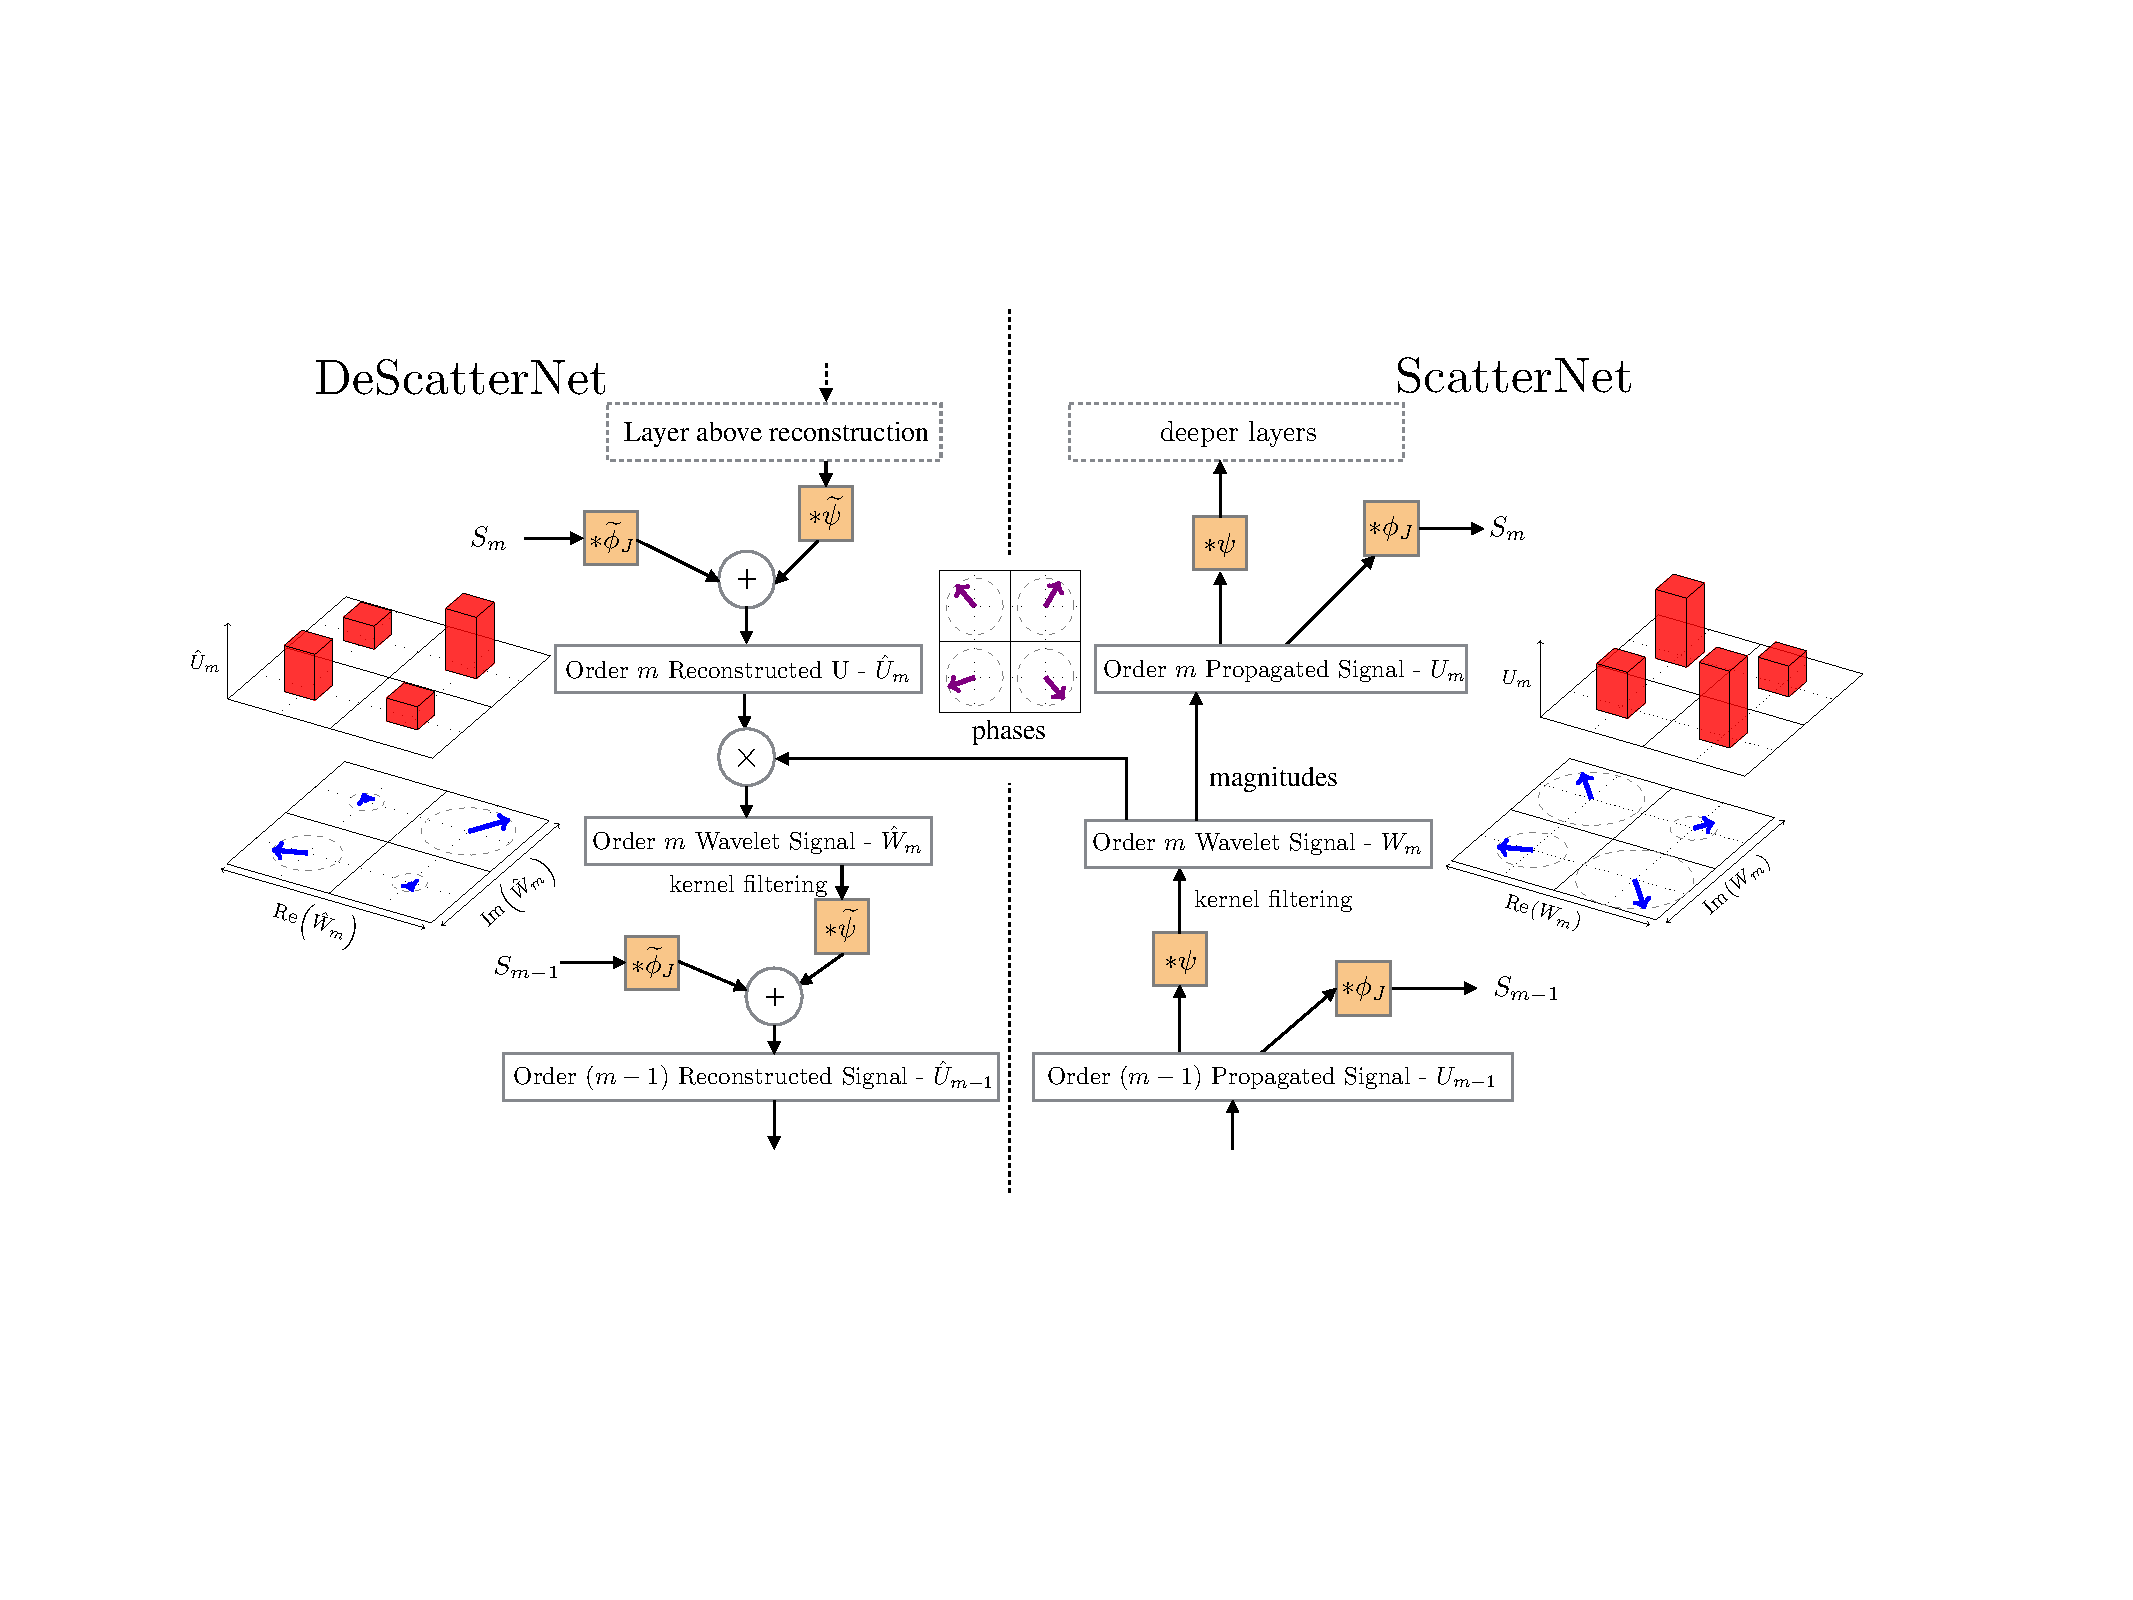
\includegraphics[width=\textwidth, trim={3cm 7cm 4cm 6cm},clip]{\imgpath/descat.pdf}
  \mycaption{The Descattering Network}{Comprised of a DeScattering layer (left)
  attached to a Scattering layer (right).  We are using the same convention as
  \cite{zeiler_visualizing_2014} Figure 1 - i.e. the input signal starts in the
  bottom right hand corner, passes forwards through the ScatterNet (up the right
  half), and then is reconstructed in the DeScatterNet (downwards on the left
  half).  The DeScattering layer will reconstruct an approximate version of the
  previous order's propagated signal. The $2\x 2$ grids shown around the image
  are either Argand diagrams representing the magnitude and phase of small
  regions of \emph{complex} (De)ScatterNet coefficients, or bar charts showing
  the magnitude of the \emph{real} (De)ScatterNet coefficients (after applying
  the modulus non-linearity). For reconstruction, we need to save the discarded
  phase information and reintroduce it by multiplying it with the reconstructed
  magnitudes.}
  \label{fig:ch4:descat}
\end{figure}

We now introduce our inverse scattering network. This allows us to back-project
scattering coefficients to the image space; it is inspired by the
DeconvNet used by Zeiler and Fergus in
\cite{zeiler_visualizing_2014} to look into the deeper layers of CNNs. Like
the DeConvNet, the inverse Scattering Network is similar to backpropagating a
single strong activation (rather than usual gradient terms). 

We emphasize that instead of thinking about perfectly reconstructing $x$ from
$S\in \reals[C\x H'\x W']$, we want to see what signal/pattern in the input image caused
a large activation in each channel. This gives us a good idea of what each
output channel is sensitive to, or what it extracts from the input. 
Note that we do not use any of the log normalization layers described in
\cite{oyallon_deep_2015, singh_dual-tree_2017}.

\subsection{Inverting the Low-Pass Filtering}
Going from the $U$ coefficients to the $S$ coefficients in the forward pass involved convolving by
a low pass filter $\phi_J$, possibly followed by decimation to make the output $(H\x
2^{-J})\x (W\x2^{-J})$.  $\phi_J$ is a purely real filter, and we can `invert'
this operation by interpolating $S$ to the same spatial size as $U$ and convolving with
the mirror image of $\phi_J$, $\widetilde{\phi}_J$ (this is equivalent to the
transpose convolution described in \cite{zeiler_visualizing_2014}). 
\begin{equation}
  \label{eq:ch4:s_hat}
  \hat{S}_{m} = S_{m} \conv \widetilde{\phi}_J
\end{equation}
This will not recover $U$ as it was on the forward pass, but will recover all
the information in $U$ that caused a strong response in $S$. We note that
interpolation usually involves lowpass smoothing of the signal, so this can all
be one operation.
% However this has
% the undesirable effect of creating multiple impulses in the next layer down's
% activations. When the next layer down is the image space this is not a problem,
% but when it is 

\subsection{Inverting the Magnitude Operation}
In the same vein as \cite{zeiler_visualizing_2014}, we face a difficult
task in inverting the non-linearity in our system. 
% It has been proven that for
% particular wavelets, we can recover the phase from their modulus
% \cite{waldspurger_phase_2012}, but this is not a trivial operation. Instead, we
We lend inspiration from the switches introduced in the DeconvNet; the
switches in a DeconvNet save the location of maximal activations so that
on the backwards pass activation layers could be unpooled trivially. We do an
equivalent operation by saving the phase of the complex activations. On the
backwards pass we reinsert the phase to give our recovered $W$. 
\begin{equation}
  \label{eq:ch4:w_hat}
  \hat{W}_{m} = \hat{U}_{m}e^{j\theta_{m}}
\end{equation}

\subsection{Inverting the Wavelet Decomposition}
Using the $\DTCWT$ makes inverting the wavelet transform simple, as we
can simply feed the coefficients through the synthesis filter banks to regenerate
the signal. For complex $\psi$, this is convolving with the conjugate transpose
$\widetilde{\psi}$: 

\begin{eqnarray}
  \label{eq:ch4:x_hat}
  \hat{U}_{m-1} &=& \hat{S}_{m-1} + \hat{W}_{m} \\
              &=& S_{m-1} \conv \widetilde{\phi}_J + \sum_{j, \theta} W_{m}(\bm{u}, j,
  \theta) \conv \widetilde{\psi}_{j, \theta}
\end{eqnarray}

\begin{figure}[tp]
  \centering
  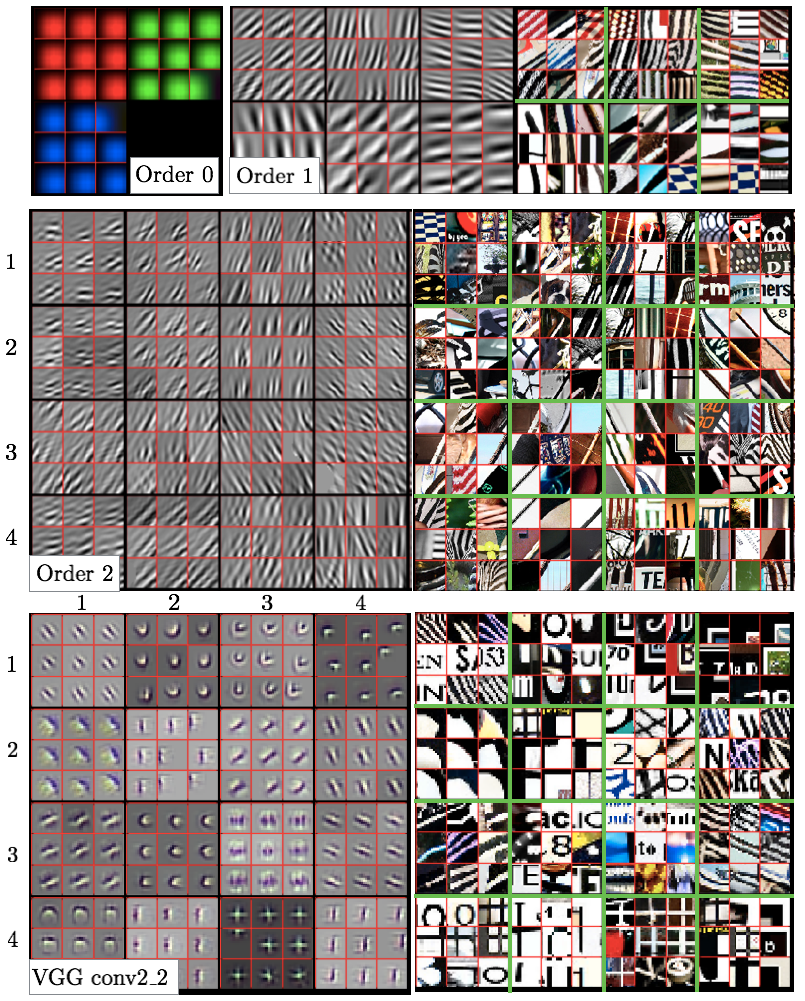
\includegraphics[width=0.9\textwidth]{\imgpath/deconv_images.png}
  \mycaption{Comparison of Scattering to Convolutional features}{Visualization
  of a random subset of features from $S_0$ (all 3), $S_1$ (6 from the 12) and
  $S_2$ (16 from the 36) scattering outputs. We record the top 9 activations for
  the chosen features and project them back to the pixel space. We show them
  alongside the input image patches which caused the large activations. We also
  include reconstructions from layer conv2\_2 of VGG Net
  \cite{simonyan_very_2014}(a popular CNN, often used for feature extraction)
  for reference --- here we display 16 of the 128 channels. The VGG
  reconstructions were made with a CNN DeconvNet based on
  \cite{zeiler_visualizing_2014}. Image best viewed digitally.}
  \label{fig:ch4:reconstructions}
\end{figure}

\section{Visualization with Inverse Scattering}
\label{sec:ch4:visualization}

To examine our ScatterNet, we scatter all of the images from ImageNet's validation
set and record the top 9 images which most highly activate each of the $C$
channels in the ScatterNet. This is the \emph{identification} phase (in which no
inverse scattering is performed). 

Then, in the \emph{reconstruction}
phase, we load in the $9\x C$ images, and scatter them one by one. We take the
resulting 52 channel output vector and mask all but a single value (usually the
largest) in the channel we are currently examining and all values in the other
channels.

This 1-sparse tensor is then presented to the inverse scattering network from
\autoref{fig:ch4:descat} and projected back to the image space. Some results of this
are shown in \autoref{fig:ch4:reconstructions}. This figure shows reconstructed
features from the layers of a ScatterNet. For a given output channel, we show
the top 9 activations projected independently to pixel space. For the first and
second order coefficients, we also show the patch of pixels in the input image
which cause this large output. We display activations from various scales
(increasing from first row to last row), and random orientations in these
scales. 

The order 1 scattering (labelled with `Order 1' in
\autoref{fig:ch4:reconstructions}) coefficients look quite similar to the first
layer filters from the well known AlexNet CNN \cite{krizhevsky_imagenet_2012}.
This is not too surprising, as the first order scattering coefficients are
simply a wavelet transform followed by average pooling. They are responding to
images with strong edges aligned with the wavelet orientation. 

The second order coefficients (labelled with `Order
2' in \autoref{fig:ch4:reconstructions}) appear very similar to the order
1 coefficients at first glance.
They too are sensitive to edge-like features, and some of them (e.g.\ third row,
third column and fourth row, second column) are mostly just that. These are
features that have the same oriented wavelet applied at both the first and
second order.  Others, such as the nine in the top left square (first row, first column), 
and top right square (first row, fourth column) are more sensitive to
checker-board like patterns. Indeed, these are activations where the orientation
of the wavelet for the first and second order scattering were far from each
other ($15\degs$ and $105\degs$ for the first row, first column and $105\degs$
and $45\degs$ for the first row, fourth column).

For comparison, we include reconstructions from the second layer of the
well-known VGG CNN\@ (labelled with `VGG conv2\_2', in
\autoref{fig:ch4:reconstructions}). These were made with a DeconvNet, following the
same method as \cite{zeiler_visualizing_2014}. Note that while some of
the features are edge-like, we also see higher order shapes like corners,
crosses and curves.

These reconstructions show that the features extracted from ScatterNets vary
significantly from those learned in CNNs after the first order. In many
respects, the features extracted from a CNN like VGGNet look preferable for use
as part of a classification system.

% \subsection{Hybrid ScatterNet Visualization}
% Visualize some of the features of a convnet.
% \pagebreak
% References should be produced using the bibtex program from suitable
% BiBTeX files (here: strings, refs, manuals). The IEEEbib.bst bibliography
% style file from IEEE produces unsorted bibliography list.
% -------------------------------------------------------------------------
